\documentclass[11pt, a4paper]{article}
\usepackage{graphicx,wrapfig}
\usepackage[margin=2cm]{geometry}
\usepackage[acronym]{glossaries}
\usepackage[sorting=none, style=nature]{biblatex} %Imports biblatex package
\usepackage[hidelinks]{hyperref}
\usepackage{titling}
\usepackage{float}
\usepackage{caption}
\usepackage{subcaption}
\usepackage{enumitem}
\usepackage{algorithm2e}
\usepackage[percent]{overpic}

\renewcommand{\familydefault}{\sfdefault}
\newcommand{\customcite}[2]{\mbox{
  {\small \copyright} \textit{#1} \cite{#2}}
}

\newcommand{\subtitle}[1]{%
  \posttitle{%
    \par\end{center}
    \begin{center}\LARGE#1\end{center}
    \vskip0.5em}%
}

\hypersetup{
  colorlinks   = true, %Colours links instead of ugly boxes
  urlcolor     = blue, %Colour for external hyperlinks
  linkcolor    = blue, %Colour of internal links
  citecolor   = red %Colour of citations
}

\addbibresource{references.bib} %Import the bibliography file

\makenoidxglossaries
\loadglsentries{glossary.tex}



\title{\textbf{ \\{\Huge Compte Rendu de Stage Master 2}}}
\subtitle{Galaxies Pop III, premières phases de la formation des métaux et poussières dans l'Univers à très grand Redshift (6 $<$ z $<$ ?)}
\author{Dewachter Tim}
\date{25 Mars 2024 - 28 Juin 2024}

\begin{document}

\maketitle

\newpage
\begin{center}
  \vspace*{\fill}

  Déclaration d'intégrité relative au plagiat \\

  

  Je soussigné \textbf{Dewachter Tim} certifie sur l'honneur : \\

  \begin{itemize}
    \centering
    \item Que les résultats décrits dans ce rapport sont l'aboutissement de mon travail ;\\
    \item Que je suis l'auteur de ce rapport ;\\
    \item Que je n'ai pas utilisé des sources ou résultats tiers sans clairement les citer et les référencer selon les règles bibliographiques préconisées.\\
  \end{itemize}

  Je déclare que ce travail ne peut être suspecté de plagiat. \\


  Date : \today\\

  

  Signature : Dewachter

  \vspace*{\fill}
\end{center}
\newpage

\tableofcontents

\newpage

\section{Introduction}

\subsection{Contexte}

\begin{wrapfigure}{r}{10cm}
  \centering
  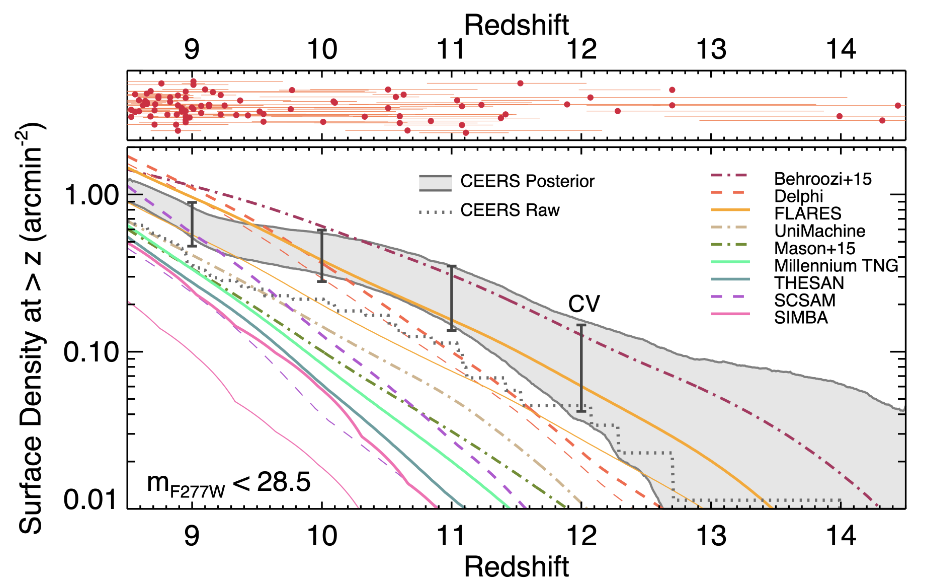
\includegraphics[scale=0.5]{assets/ceers_number_galaxies.png}
  \caption{Comparaisons modèles - données de la densité du nombre de galaxies en fonction du redshift. En haut, les différents redshifts mesurés avec leurs incertitudes. En bas, Les traits colorés représentent différents modèles pré-JWST, tandis que la zone grisée représente les données obtenues par le programme CEERS. Seuls 2 modèles semblent en accord avec les données. \customcite{Finkelstein et al.}{2023arXiv231104279F}}
  \label{fig:densite_galaxies}
\end{wrapfigure}

En seulement 2 ans d'opérations, le \gls{jwst} nous a déjà ouvert de nombreuses portes jusqu'alors inaccessibles, et cela dans de multiples branches de l'astrophysique. Grâce à ses instruments spectroscopiques et sa sensibilité à l'infrarouge proche et moyen, il est désormais possible de sonder l'univers comme jamais auparavant. Parmi les objectifs que l'on souhaite accomplir avec ce télescope, l'un d'eux est l'étude de la formation des galaxies à l'époque de la réionisation, de l'apparition des métaux au sein de celles-ci, et de la recherche des hypothétiques Populations III, constituées d'étoiles de métallicité nulle, formées par le gaz primordial d'Hydrogène et d'Hélium purs.

Ce nouvel horizon sur l'univers lointain nous permet de remonter l'histoire de l'univers comme jamais auparavant. En effet, la vitesse finie de la lumière fait que regarder loin dans l'espace est équivalent à remonter dans le temps. À cela s'ajoute également l'expansion de l'univers, avec pour conséquence de décaler le spectre lumineux de ces objets lointains vers le rouge (on parle de redshift).

D'ores et déjà, de nombreux résultats remettent en question nos modèles précédemment établis. L'un d'eux, notamment, est qu'il semblerait qu'il existe bien plus de galaxies dans l'univers jeune que ce que l'on pensait jusqu'à présent \cite{2023arXiv231104279F} (voir figure \ref{fig:densite_galaxies}). Un autre est la découverte d'un potentiel candidat de Population III \cite{2023arXiv230600953M}, où une raie d'He II à $\lambda = 1640 \text{\r{A}}$ semble indiquer qu'un nuage de gaz à $z = 10.6$ s'est retrouvé ionisé par des étoiles de Pop III. 

Ainsi, dans les années à suivre, il est certain que de nouvelles contraintes vont pouvoir être posées sur les modèles de formation des premières galaxies et sur l'évolution de leur metallicité grâce au JWST.

\subsection{Problématiques et Objectifs}

Comment peut-on utiliser la spectroscopie comme outil pour sonder les paramètres physiques des premières galaxies ?\\

Nous allons par la suite traiter ce problème en 2 parties.

Tout d'abord, nous étudierons le code de traitement des données du \gls{jwst} dans le but de modifier son algorithme de soustraction du fond, afin d'en extraire les éventuels faibles spectres de sources secondaires jusqu'alors dissimulés dans le fond.

Ensuite, nous étudierons ces différents spectres via \gls{cigale} afin d'en déterminer les paramètres physiques, telles que leur redshift, leur metallicité ou leur taux de formation stellaire.

\section{Méthodologie}

\subsection{JWST et NIRSpec}

\begin{figure}
  \centering
     \begin{subfigure}[b]{0.45\textwidth}
         \centering
         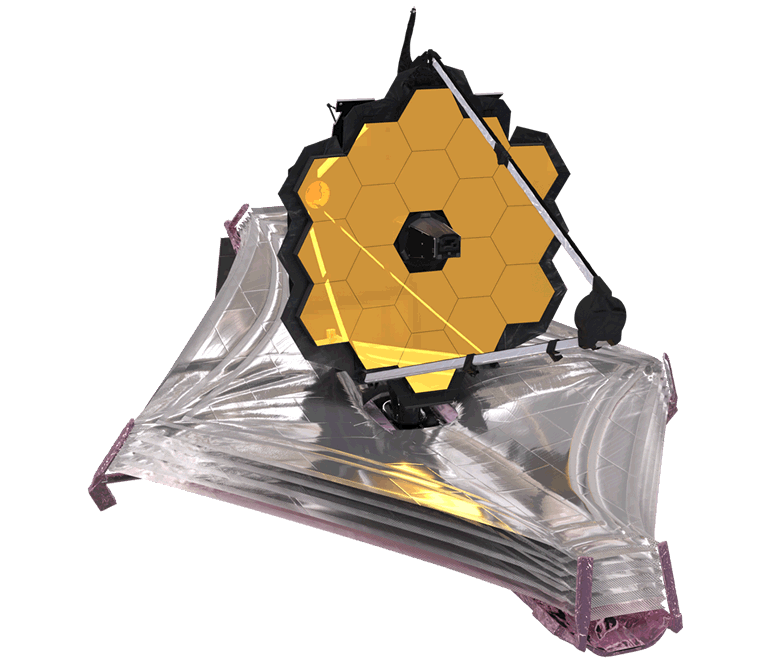
\includegraphics[width=\textwidth]{assets/JWST_spacecraft_model_3.png}
         \caption{Rendu 3D du \gls{jwst}. \customcite{NASA}{jwst_nasa}}
         \label{fig:jwst}
     \end{subfigure}
     \hfill
     \begin{subfigure}[b]{0.45\textwidth}
         \centering
         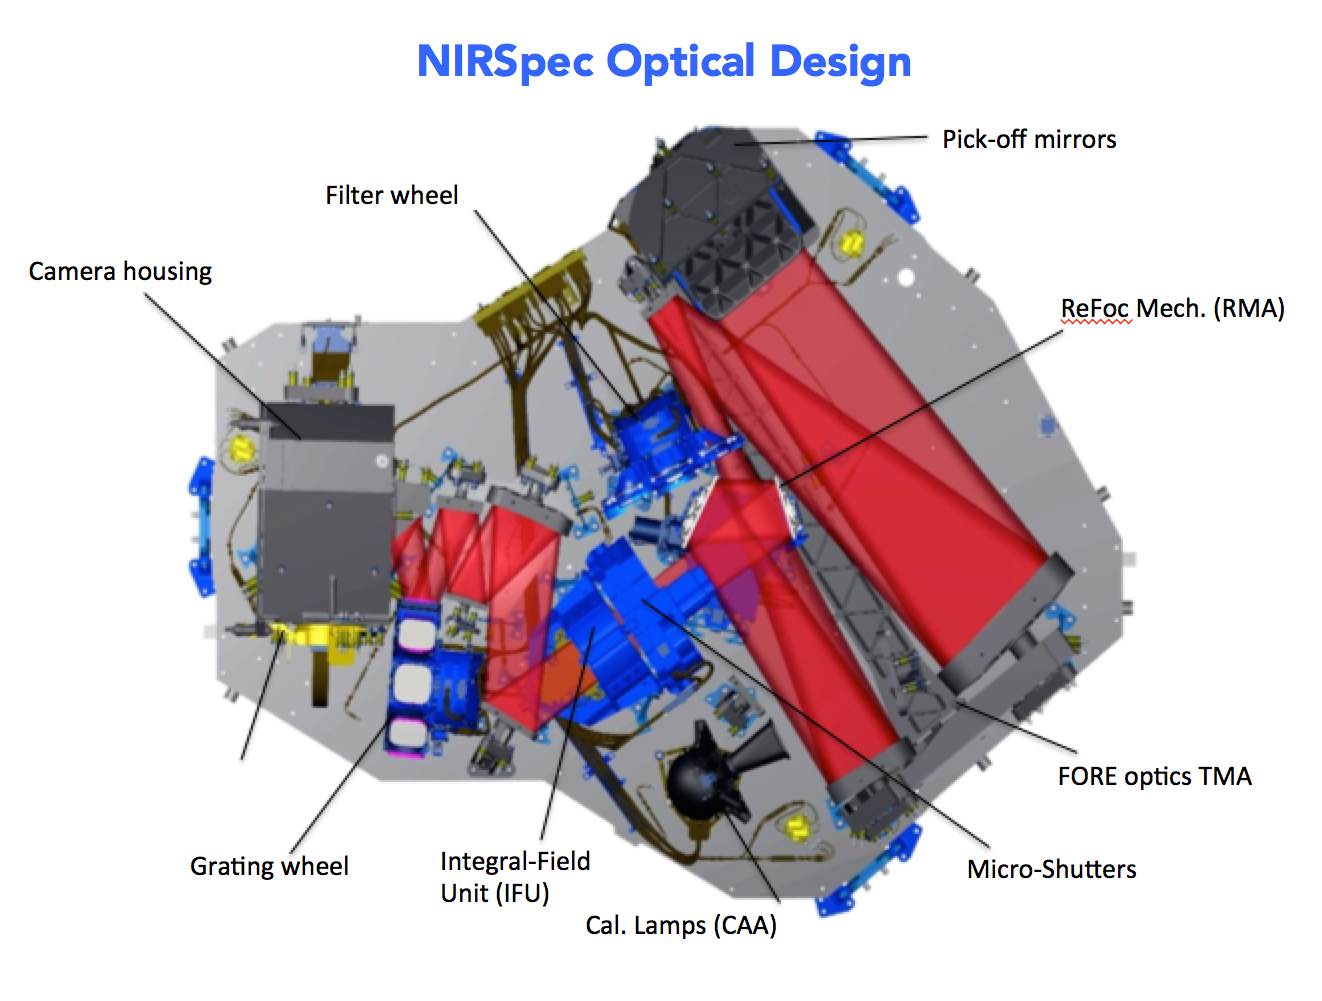
\includegraphics[width=\textwidth]{assets/NIRSpec_Optical_design.png}
         \caption{Schéma des optiques de \gls{nirspec}. \customcite{STScI}{nirspec}}
         \label{fig:nirspec}
     \end{subfigure}
\end{figure}

Le \gls{jwst} est un télescope spatial de 6.5 mètres de diamètre équivalent, en orbite autour du point de Lagrange L2, et actif depuis juillet 2022 \cite{jwst_website}. Sa sensibilité dans l'infrarouge en fait un outil remarquable pour observer l'univers jeune. En effet, de par l'expansion de l'univers, la lumière des objets lointains se retrouve décalée vers le rouge : il s'agit du redshift $z$, défini comme 

\begin{equation}
    1 + z = \frac{\lambda_{obs}}{\lambda_{rest}}
\end{equation}

Avec $\lambda_{obs}$ la longueur d'onde observée, et $\lambda_{rest}$ la longueur d'onde dans le référentiel de la source (au repos). Ainsi, regarder loin dans l'espace est équivalent à regarder loin dans le passé et nécessite d'observer à des longueurs d'ondes de plus en plus grandes.

\begin{figure}[!h]
  \centering
  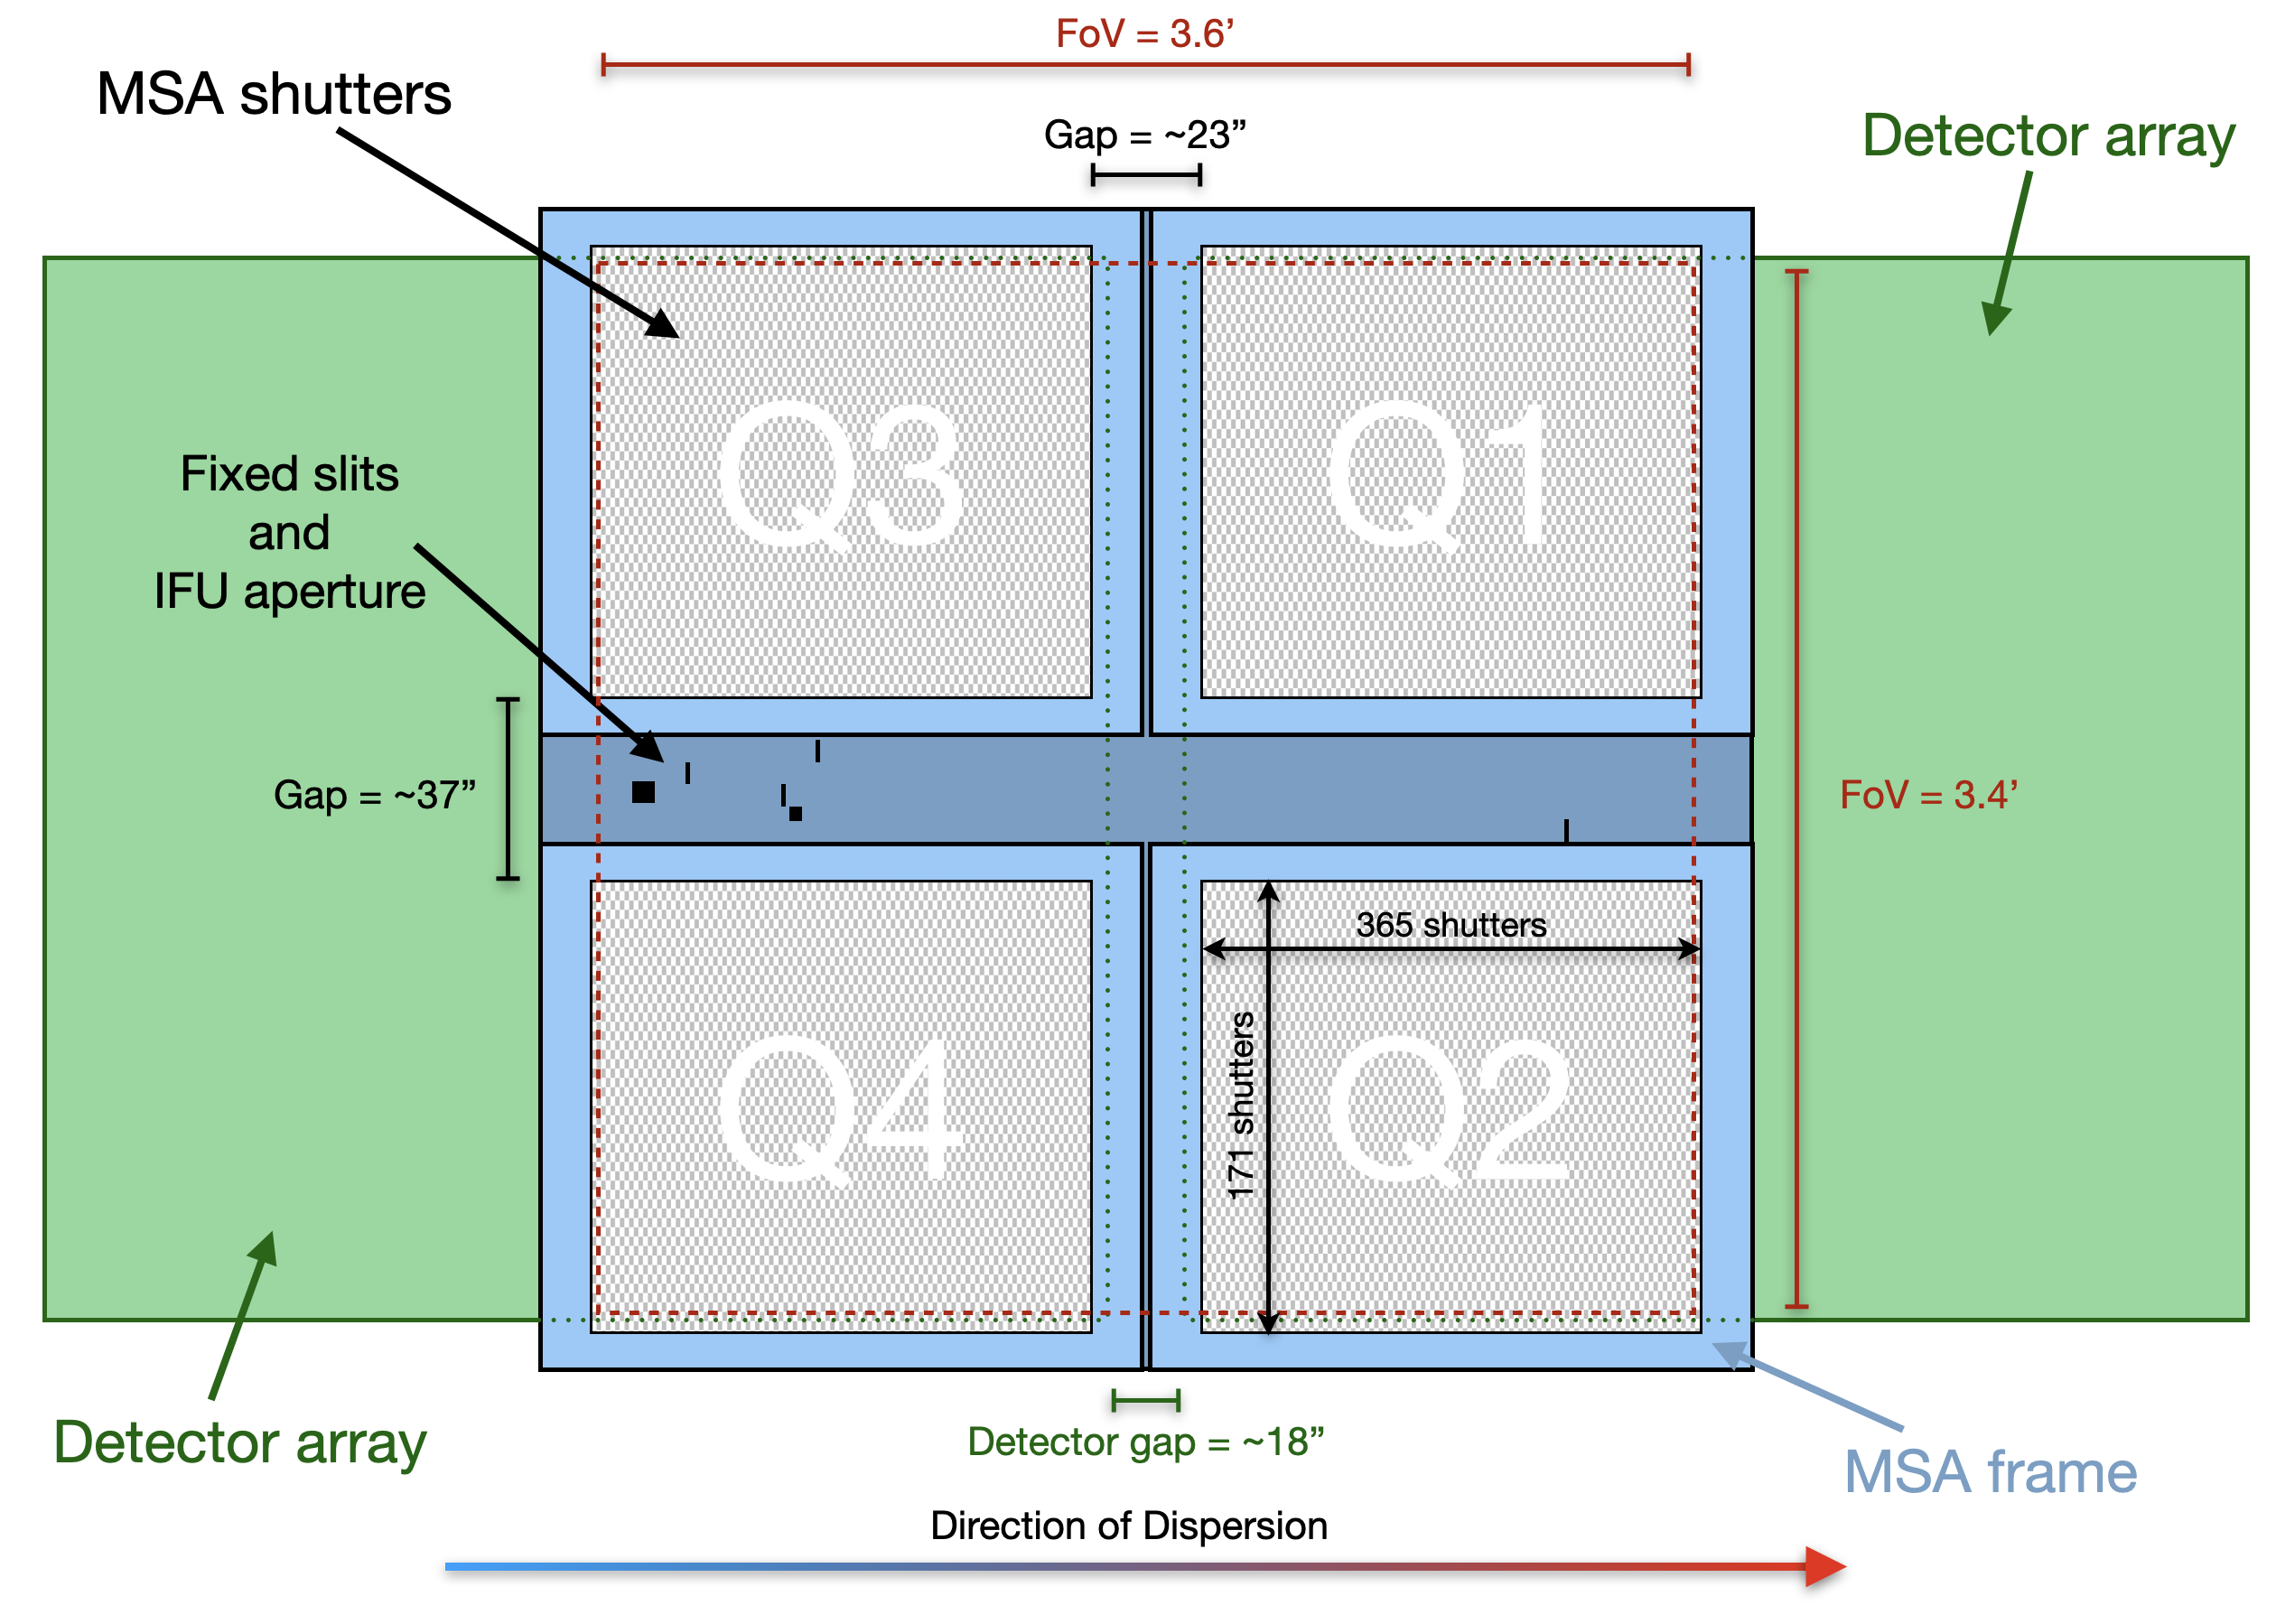
\includegraphics[scale=0.3]{assets/msa_ds_new.png}
  \caption{Disposition de MSA dans le plan focal de NIRSpec. \customcite{Ferruit et al.}{2022A&A...661A..81F}}
  \label{fig:msa_shutter}
\end{figure}

Parmi les instruments du \gls{jwst}, \gls{nirspec} est un spectromètre sur la bande 0.6 - 5.3  µm, disposant de 3 modes de résolution : PRISM ($R \sim 100$), medium grating ($R \sim 1000$), high grating ($R \sim 2700$) \cite{nirspec}. L'un des atouts principaux de \gls{nirspec} est son \gls{msa}, une grille de près de 250 000 obturateurs, couvrant une surface de 3.6' x 3.4' sur le ciel, chacun pouvant être individuellement ouvert ou fermé \cite{msa} (voir \ref{fig:msa_shutter}). Ceci permet d'observer dans le mode \gls{mos} de \gls{nirspec}. Comme son nom l'indique, la spectroscopie multi-objet permet d'étudier le spectre de plusieurs objets dans un même champ, mais la grille d'obturateurs apporte également un outil fondamental dans l'extraction des spectres : la soustraction du fond.\\

Nous travaillerons ici sur des données \gls{nirspec} du Programme de \textit{The Cosmic Evolution Early Release Science (CEERS)}, disponibles sur la base de données MAST \cite{portal_mast} (Proposal ID : 1345), notamment les observations P4, P5, P7, P8, P9, P11, P12, avec comme résolution PRISM.

\subsection{Fond, Nodding et Slitlet}

Lorsqu'on s'intéresse à des sources de faible brillance, le flux lumineux mesuré peut rapidement se trouver dominé par les émissions du fond. Que ce soit le fond diffus infrarouge, produit par des sources extragalactiques non résolues, la lumière zodiacale, produite par la poussière interplanétaire, le rayonnement de la Voie Lactée ou l'émission thermique du JWST lui-même, l'infrarouge est un domaine facilement parasité par des signaux indésirables \cite{jwst_background}. De plus, la nature de ses composantes fait de ce fond un signal anisotrope. Il n'est donc pas si simple d'en établir un modèle universel à soustraire de façon systématique. On a la mesure du fond en fonction de la longueur d'onde ci-dessous \ref{fig:background_jwst} : 

\begin{figure}[!h]
  \centering
  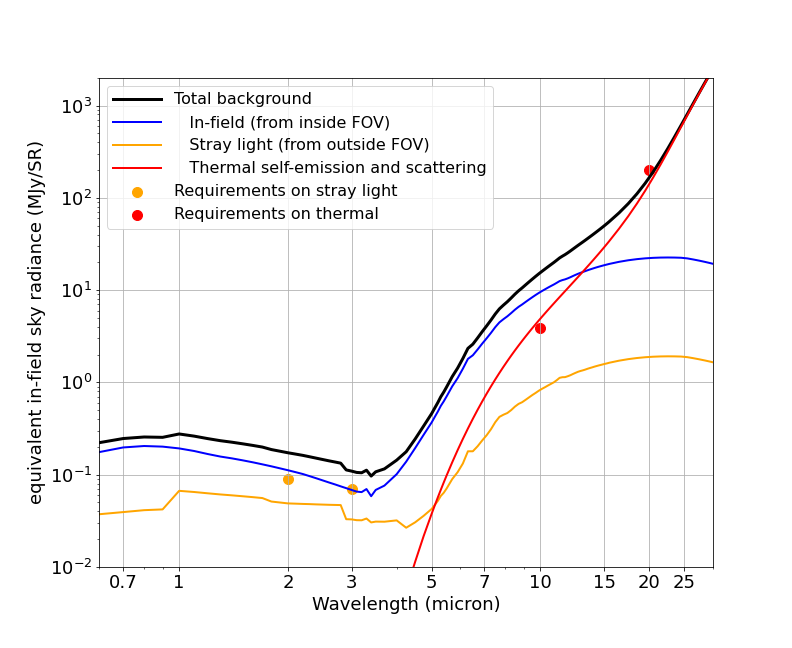
\includegraphics[scale=0.55]{assets/background_jwst.png}
  \caption{Flux par unité d'angle solide reçu par le JWST en fonction de la longueur d'onde. On remarque qu'à mesure que $\lambda$ augmente, l'émission thermique du télescope domine. \customcite{STScI}{jwst_background}}
  \label{fig:background_jwst}
\end{figure}


Cependant, il reste tout de même envisageable de corriger ce signal parasite. En effet, en ouvrant les obturateurs à proximité de celui imageant la source, il devient possible d'extraire le fond localement autour de la source, que l'on peut alors soustraire au spectre de cette dernière.

La configuration habituelle consiste en l'ouverture de 3 obturateurs dans la direction perpendiculaire à la direction de dispersion. Dans un souci de cohérence avec la documentation du pipeline, on parlera par la suite de \textit{Slitlet}. On réalise alors 3 expositions, chacune en orientant le télescope de façon à avoir la source dans un obturateur différent : il s'agit du nodding. Ce mouvement entre chaque exposition offre également un autre avantage au travers du \textit{dithering}. La \gls{psf} de \gls{nirspec} est effectivement de $0.08 ''$ à $\lambda = 2.46 \mu m$ \cite{10_1051_0004_6361_202142663}. 
Comme $PSF \propto \lambda$, on a une \gls{psf} variant de $0.02 ''$ à $0.17''$ le long de la plage de longueur d'onde observable. Comme la taille d'un pixel est $\sim 0.1''$ dans la direction spatiale, la \gls{psf} est sous échantillonnée presque partout. Le dithering permet alors d'améliorer cet échantillonnage par des corrections sub-pixels, mais également de s'affranchir des éventuels pixels défectueux ou des rayons cosmiques.

On résume ceci dans la figure \ref{fig:msa_slitlet}.


\begin{figure}[H]
  \centering
  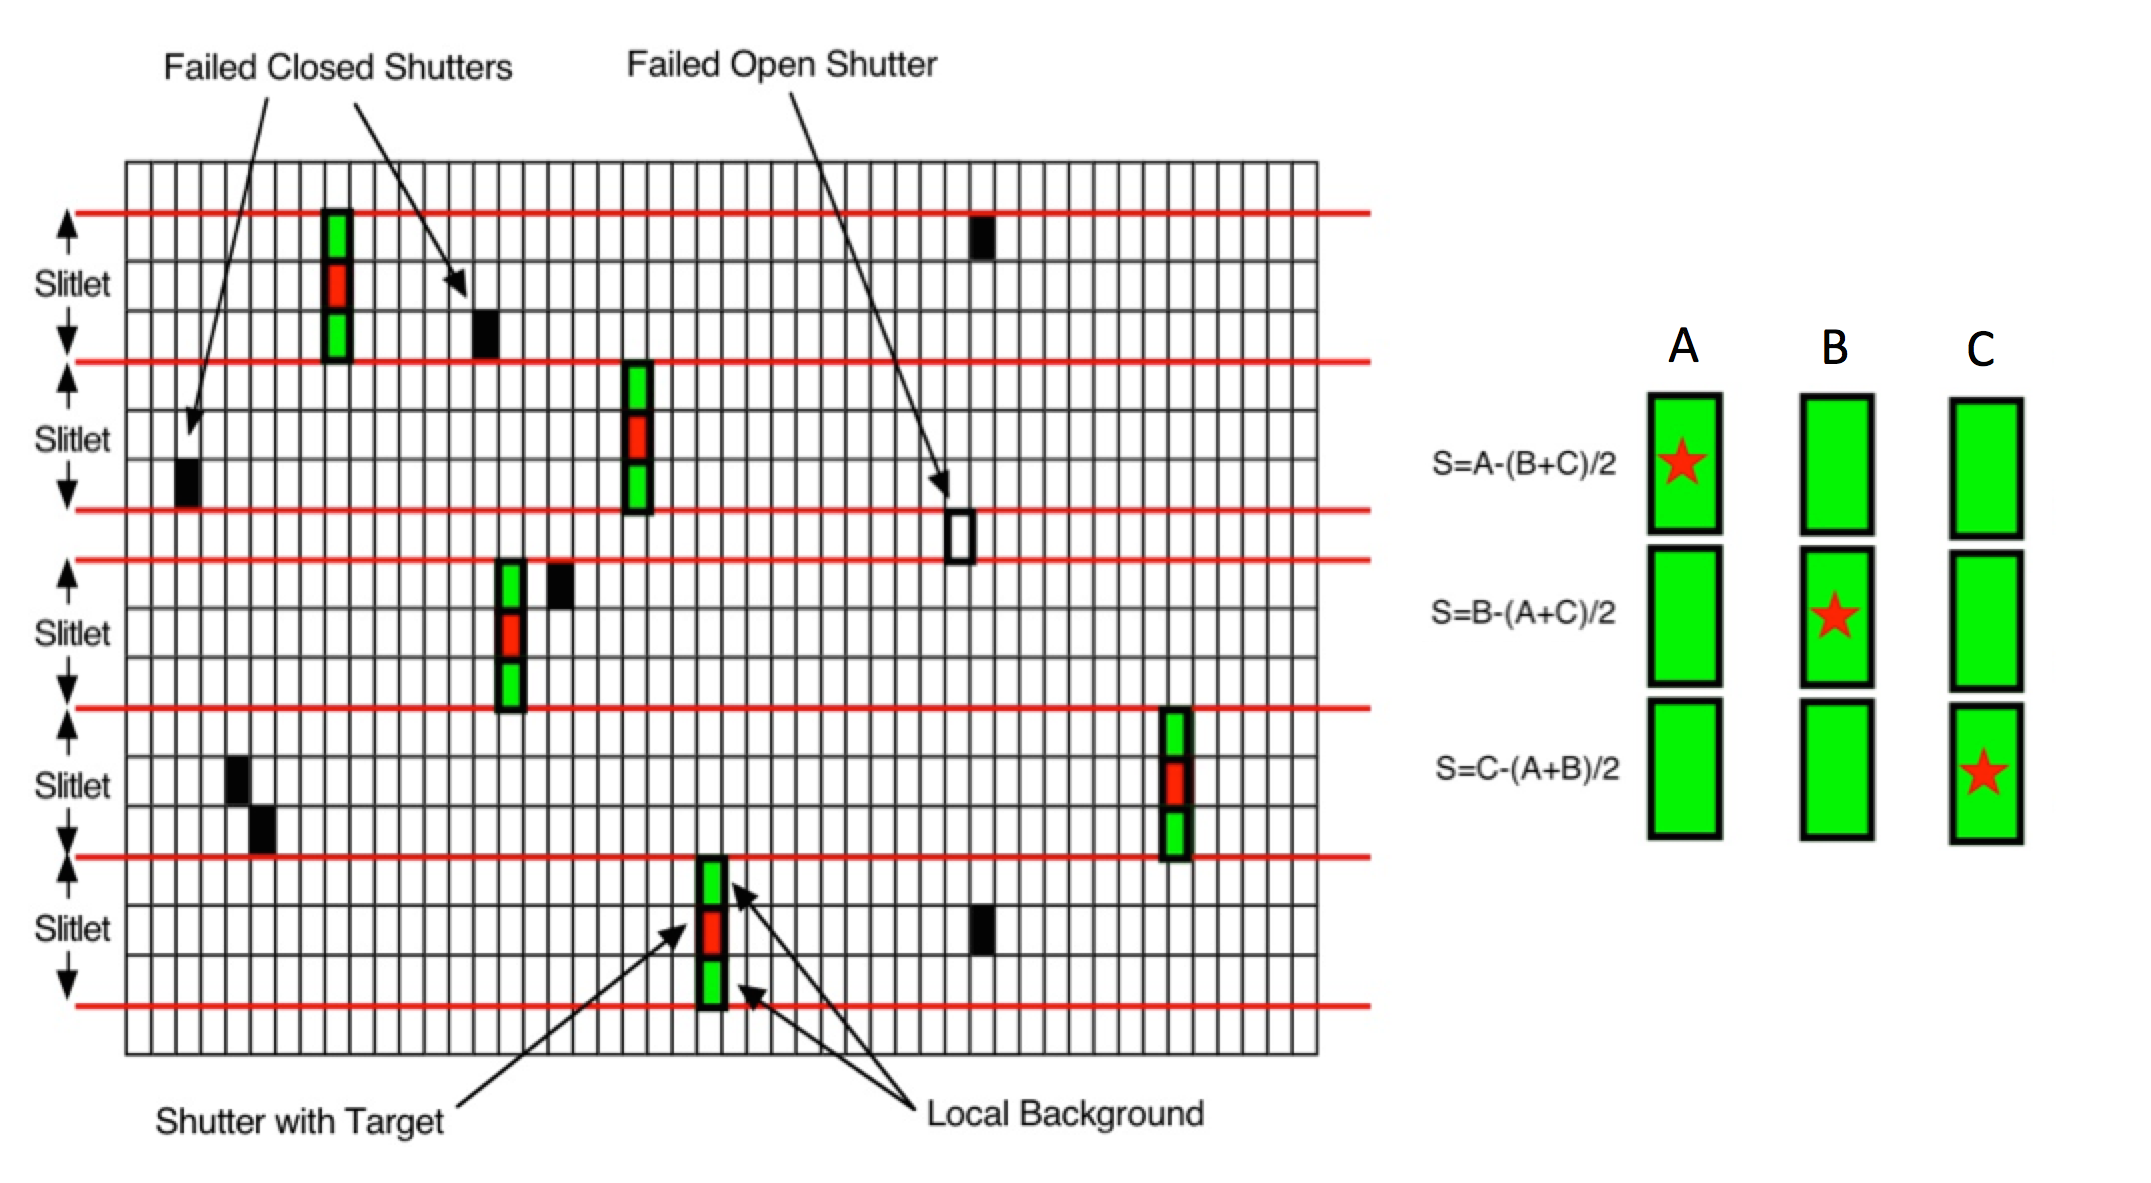
\includegraphics[scale=0.2]{assets/MSA_sky_strategy.png}
  \caption{Schéma de MSA et de slitlets. On réalise des séries de 3 images, chacune ayant la source dans un obturateur différent, et on utilise les 2 obturateurs restant pour déterminer le spectre du fond. \customcite{NIRSpec Instrument Development Team}{mos}}
  \label{fig:msa_slitlet}
\end{figure}

\subsection{Le pipeline JWST}

Le code permettant de traiter les données reçues du JWST, appelé pipeline (figure \ref{fig:jwst_pipeline}), se décompose en 3 grandes étapes, celles ci étant de plus en plus spécifique aux types de données que l'on cherche à étudier à mesure que l'on progresse dans le pipeline.

Ainsi, dans notre cas, les 3 étapes sont telles que :\\


\begin{minipage}{.45\linewidth}
  \begin{itemize}[left=0cm]
    \item \textbf{Detector 1} : Applique les corrections au niveau du détecteur, tel que le masquage des pixels morts/chauds et des rayons cosmiques, la linéarisation du nombre de détections par seconde, la suppression du biais et du courant d'obscurité... Cette étape est la même pour tous les instruments du \gls{jwst}. (cf. \ref{fig:rate_file} le fichier en sortie de cette étape)
    \item \textbf{Spectroscopy 2} : Applique des modifications optiques, telles que la correction de champ plat et des pertes de lumières liées aux barres séparant les obturateurs, mais calibre également la photométrie et les données \gls{wcs}, associant à chaque pixel des coordonnées spatiales et spectrales. C'est ici que les images de chaque slitlets sont extraites de l'image initiale et que la soustraction du fond s'applique.
    \item \textbf{Spectroscopy 3} : Combine plusieurs expositions entre elles, appliquant ainsi le dithering / nodding discuté plus tôt, ré-échantillonne les images 2D et extrait les spectres 1D de celles-ci.
  \end{itemize}
  \end{minipage}
  \hfill
  \begin{minipage}{.5\linewidth}
  \centering
  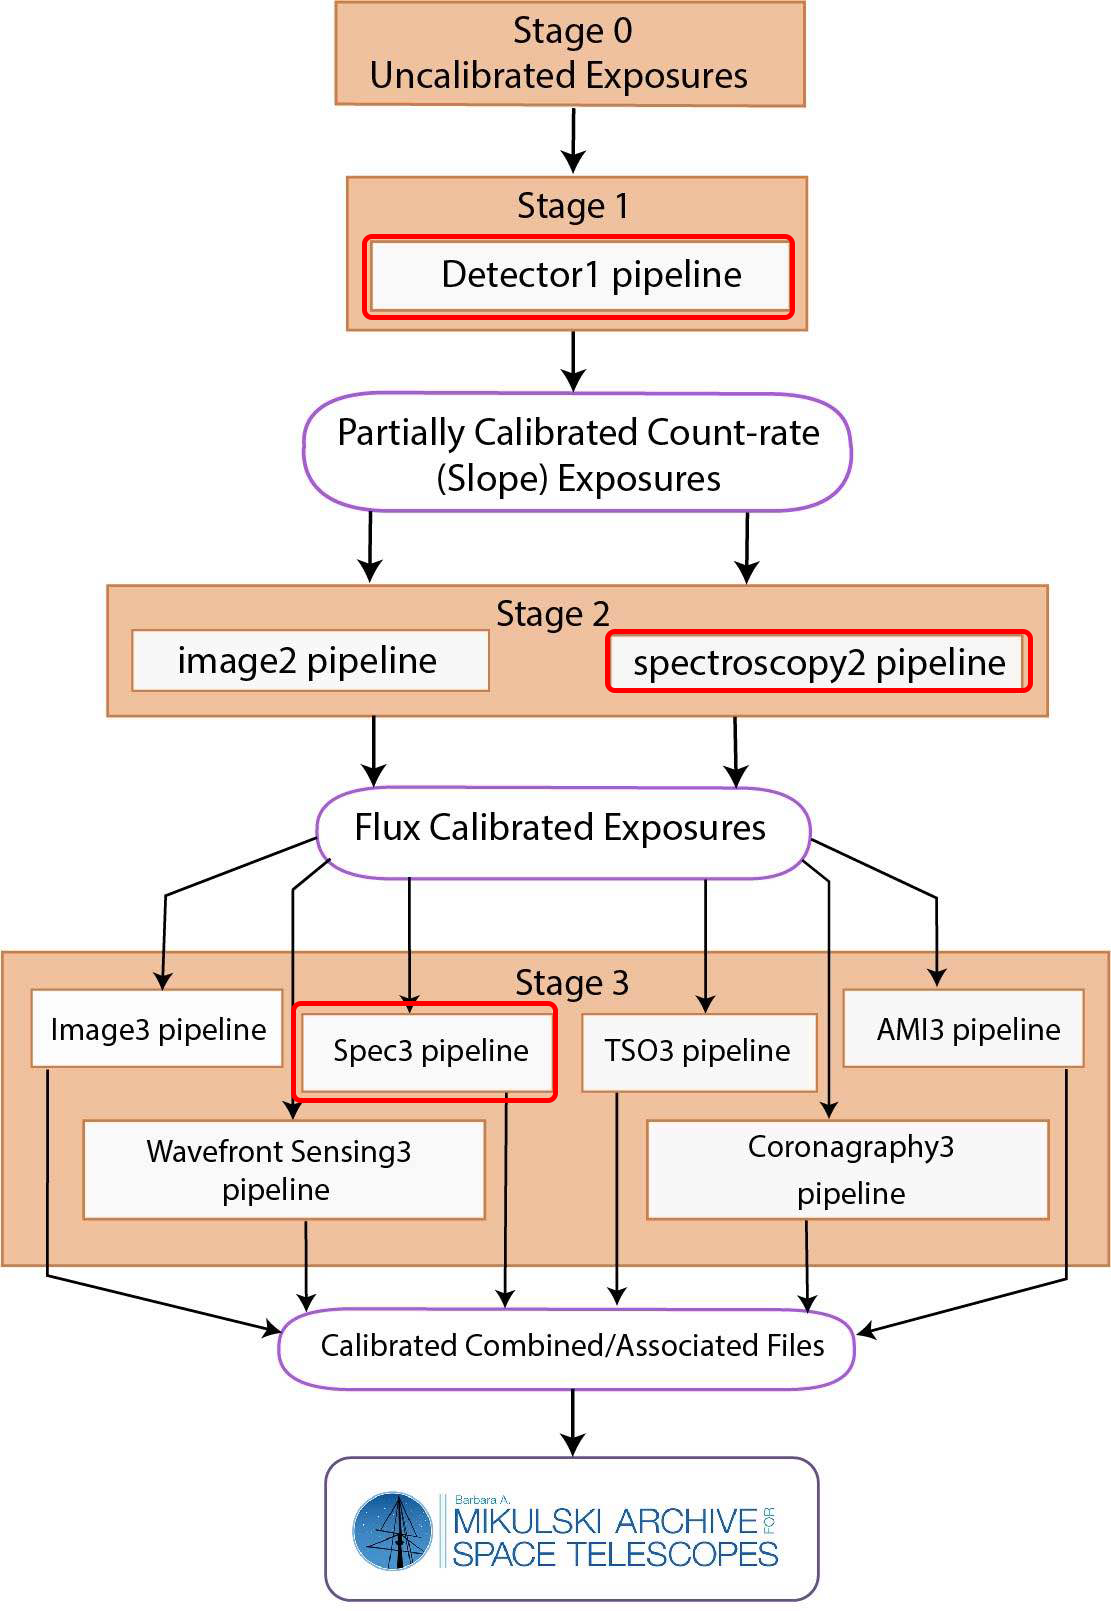
\includegraphics[scale=0.15]{assets/jwst_pipeline.jpg}
  \captionof{figure}{Schéma des différentes étapes du pipeline. Les étapes adaptées à nos données sont encadrées en rouge.\customcite{STScI}{jwst_pipeline}}
  \label{fig:jwst_pipeline}
  \end{minipage}


  \begin{figure}[H]
    \centering
    \begin{overpic}[width=1\textwidth]{assets/rate_file_illustrated.png}
      % The coordinates (x, y) specify the position of the caption text.
      % For example, (20,80) would place the caption at 20% from the left and 80% from the bottom.
      \put(52.5,13){%
          \parbox{8cm}{
            \fontsize{11}{12}\selectfont Image de \gls{nirspec} en sortie de l'étape 1 du pipeline. On peut y observer des taches lumineuses correspondant aux ordres 0 de diffraction (vert), des larges bandes au milieu formées par des obturateurs toujours ouvert, utilisé lors du mode Fixed Slit (bleu), ainsi que des bandes plus fines, parfois regroupées par 3, parfois isolées lorsqu'un obturateur reste accidentellement ouvert
          }
      }
    \end{overpic}
    \caption{}
    \label{fig:rate_file}
  \end{figure}

  \subsubsection{Soustraction du fond par défaut}

  Dans le cas de données \gls{nirspec} \gls{mos}, la soustraction du fond se fait pixel par pixel, lors de l'étape 2 du pipeline. Sur chaque slitlet, pour une exposition donnée, on considère les 2 expositions restantes comme du signal de fond, on les moyenne donc avant de les soustraire à l'image initiale. Cette étape est décrite sur la figure \ref{fig:msa_slitlet}

  Cette méthode a l'avantage majeur de permettre de soustraire le fond localement autour de la source. Cependant, celle ci se heurte à un problème dans le cas où la source est suffisamment étendue pour être visible depuis un des obturateurs de fond, ou dans celui où celle ci est mal centrée dans l'obturateur principal, mais également dans la situation plus intéressante où une autre source suffisamment brillante se situe dans le champ d'un des obturateurs de fond. Dans chacun de ces scénarios, le spectre de "fond" n'en est plus réellement un : on observe une sur-correction du spectre de l'objet. Les raies d'émission sont atténuées sur la bande de signal et des raies inversées apparaissent sur les autres bandes, en raison de la soustraction. C'est ce que l'on observe sur la figure \ref{fig:negative_trace} : les bandes au-dessus et en dessous de la bande principale présentent un spectre négatif. Cette sur-correction a également pour conséquence de cacher toute galaxie de faible luminosité se trouvant dans une des bandes du fond.\\
  
  \begin{figure}[H]
    \centering
    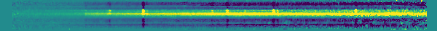
\includegraphics[scale=1.1]{assets/negative_trace_nirspec.png}
    \caption{Exemple d'une image 2D d'un spectre de \gls{nirspec} en fin de traitement classique. On observe clairement des spectres négatifs au-dessus et en dessous de la bande contenant le signal. Ceci est particulièrement visible à proximité des raies intenses.}
    \label{fig:negative_trace}
  \end{figure}

  Le pipeline offre également un autre algorithme, dit de master background, qui extrait puis combine les spectres de plusieurs obturateurs de fond, ailleurs dans le champ, avant de ré-interpoler le spectre en 2D et de le soustraire. Cette méthode, bien qu'offrant en général un meilleur rapport signal sur bruit, a le désavantage de perdre l'aspect local du fond avec la soustraction pixel par pixel.

  \subsubsection{Soustraction du fond personnalisée}

  Nous allons ici chercher à établir une nouvelle méthode de soustraction du fond, combinant le meilleur signal sur bruit du master background avec la composante locale de la soustraction pixel par pixel. L'algorithme est comme suit :\\

  \begin{algorithm}[H]
    $raw$ = données à traiter \;
    Appliquer le stage 1 du pipeline sur $raw$ \;
    Appliquer le stage 2 du pipeline sur $raw$ jusqu'à l'étape Master Background \;
    Application temporaire des étapes FlatField, PathLoss, BarShadow, Photom, ResampleSpec \;
    \ForEach{Slitlet dans $raw$}{
      \If{Nombre de shutters dans slitlet = 3}{
        Moyenne spectrale de l'image dans la direction de dispersion \;
        Détermination des positions $y_i$ de chaque bande par ajustement de 3 profils gaussien \;
        \ForEach{$i \in [1,2,3] \; \& \; i \neq source$}{
          Extraction et moyenne spatiale des $z_j^i$, les 2 bandes de fond, centrée sur $y_i$, avec une étendue spatiale de 3 pixels \;
          Extraction et moyenne spatiale des $\lambda_j^i$, longueurs d'ondes associées \;
          Extraction et moyenne spatiale des $(\sigma_j^i)^2$, les variances sur $z_j^i$ associées \;          
         }
        Ajuster une spline $f(\lambda_j^i)$ aux données $z_j^i$, de degré $k=5$ et de facteur de lissage $s=0.01$ \;
        Créer une nouvelle image $Z_{(x,y)} = f(\lambda_{(x,y)})$ \;
        Appliquer les étapes inverses de ResampleSpec, Photom, BarShadow, PathLoss, FlatField \;
        Calcul des données traitées $trait\acute{e}e_{(x,y)} = raw_{(x,y)} - Z_{(x,y)}$ \;
        }
    }
    Appliquer les étapes suivantes du stage 2 du pipeline sur $trait\acute{e}e$\;
    Appliquer le stage 3 du pipeline sur $trait\acute{e}e$\;
  \end{algorithm}

\subsection{Analyse de l'algorithme}

La méthode décrite ici est basée sur celle utilisée lors de l'étape MasterBackgroundStep du pipeline \cite{mos_master_background}.

\subsubsection{Calibration temporaire}

L'application temporaire des étapes FlatField, PathLoss, BarShadow, Photom et ResampleSpec, permet d'extraire les spectres de fond de façon plus efficace. Ces étapes sont inversées par la suite, une fois un modèle de fond calculé, cela dans le but de faciliter l'ajustement du modèle du fond.

\begin{itemize}
  \item \textbf{FlatField} : Le Flat Field, ou Champ Plat, permet de corriger les défauts optiques (débris sur les miroirs ou le détecteur, distorsions optiques...) ainsi que les variations de sensibilités de chaques pixels. Ces images de calibrations dépendent de la longueur d'onde, et il est donc nécessaire dans le cas de \gls{nirspec} d'en combiner et interpoler plusieurs afin de couvrir le domaine spectral observé. La correction est alors appliquée en divisant l'image de chaque slitlet par le champ plat.
  \begin{equation}
    \mathsf{CORRECTION} = \mathsf{SCI} \; / \; \mathsf{FLAT} 
  \end{equation}

  \item \textbf{PathLoss} : Permet de compenser les pertes de lumières dans le système optique (taille finie des obturateurs, pertes de lumière en dehors du réseau).
  
  \item \textbf{BarShadow} : Compense les pertes liées aux barres séparant les obturateurs dans le cas de sources étendues.
  
  \item \textbf{Photom} : Traitement photométrique de l'image, où celle ci passe de valeurs arbitraires en DN/s (comptage d'événements par seconde) à des valeurs physiques de flux. Le facteur de conversion dépend de la longueur d'onde et est obtenu grâce à un tableau de référence, avant d'être interpolé aux longueurs d'ondes d'intérêt.\\
  
  À la fin de cette étape, une copie des données prétraitées est réalisée. C'est depuis cette copie que les étapes inverses seront appliquées par la suite.
  
  \item \textbf{ResampleSpec} : Ré-échantillone l'image de chaque slitlet de façon à corriger toute déformation et rotation de l'image, tout en alignant la direction de dispersion spectrale sur l'axe horizontal et la direction spatiale avec l'axe vertical.
\end{itemize}

\begin{figure}[H]
  \centering
  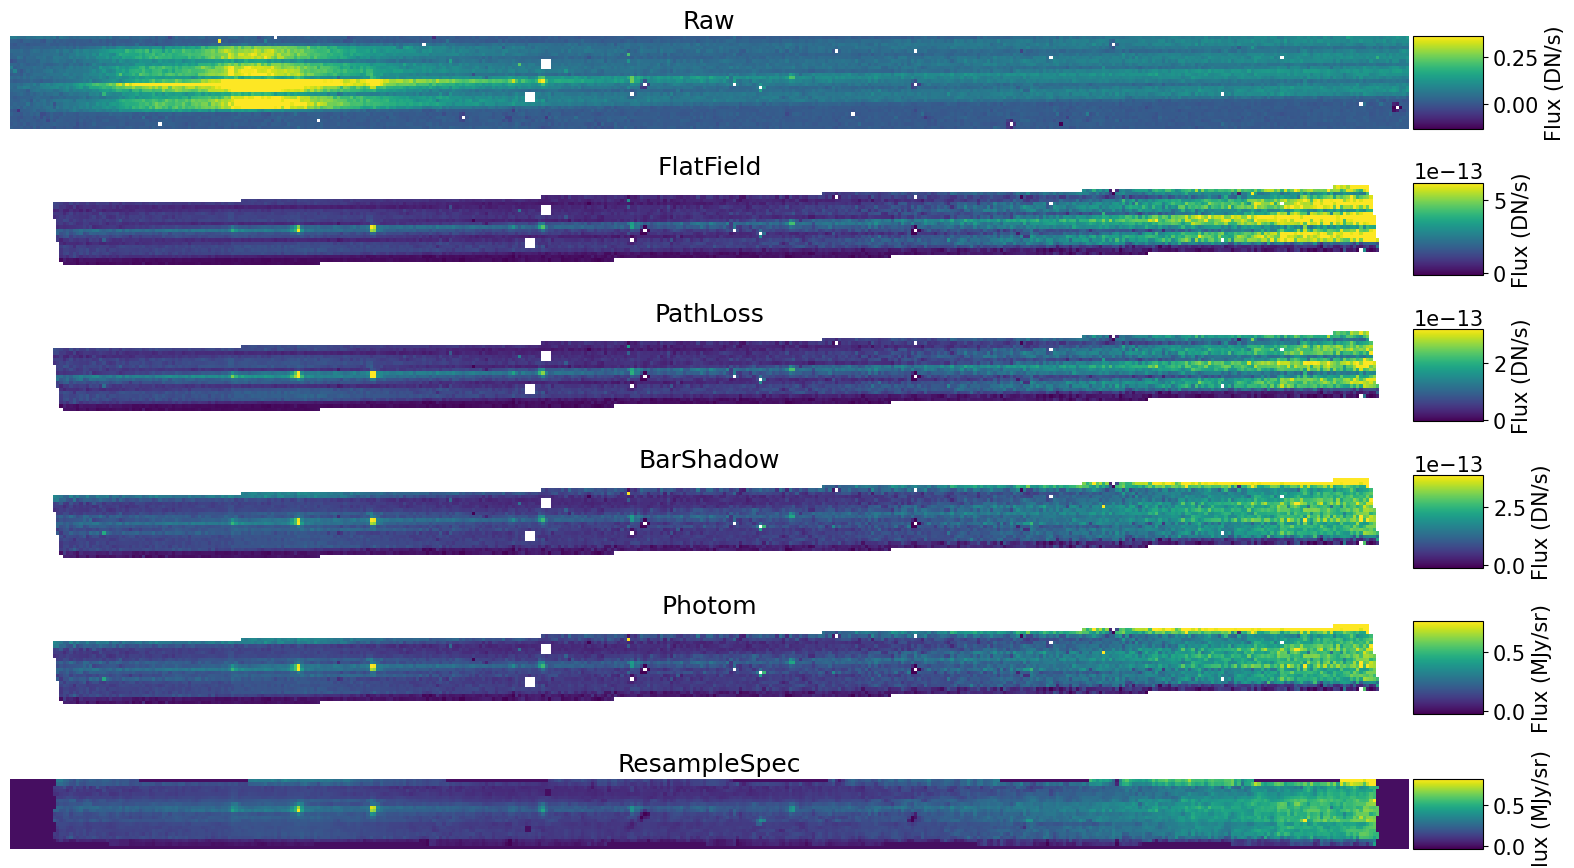
\includegraphics[scale=0.45]{assets/precal.png}
  \caption{La précalibration appliquée à l'image d'un slitlet. On remarque que le traitement par FlatField corrige grandement le flux et est effectivement inégal selon la longueur d'onde, que PathLoss et BarShadow permettent de s'affranchir de l'ombre des barres sur l'image, que Photom permet le passage de $DN/s$ (le nombre de détections par seconde) vers des $MJy/sr$, et que ResampleSpec permet de redresser l'image. Les pixels blancs sont des pixels masqués par l'algorithme, car défectueux ou présence de rayons cosmiques.}
  \label{fig:precal}
\end{figure}


\subsubsection{Détermination des positions des bandes}

\begin{wrapfigure}{r}{.5\textwidth}
  \begin{minipage}{\linewidth}
    \centering\captionsetup[subfigure]{justification=centering}
    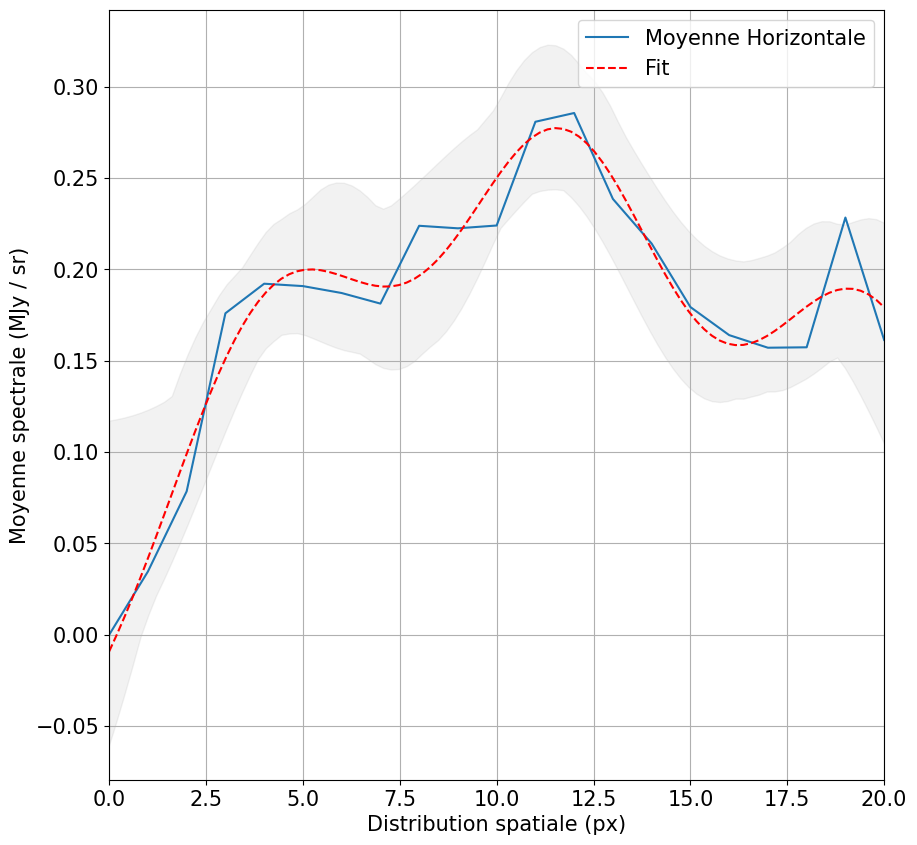
\includegraphics[width=0.9\linewidth]{assets/fit_gaussian.png}
    \subcaption{Profil de la distribution spatiale de l'image d'une slitlet après avoir moyenné sur les longueurs d'ondes. On ajuste alors ce profil par 3 gaussiennes.}
    \label{fig:profil_gauss}
    \par
    \vfill
    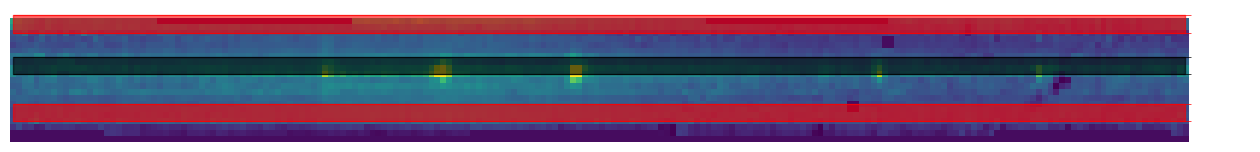
\includegraphics[width=\linewidth]{assets/extraction.png}
    \subcaption{Visualisation en rouge des zones d'extractions du fond et en noir de la zone du signal, qui ne nous intéresse pas ici.}
    \label{fig:extraction}
  \end{minipage}
\end{wrapfigure}

L'étape ResampleSpec nous permet d'être certain que la direction verticale sur l'image correspond à une dispersion spatiale, tandis que la direction horizontale correspond à une dispersion spectrale. Pour discriminer la bande contenant le signal principal de celles contenant le spectre de fond, nous réalisons donc une moyenne spectrale, tronquée à $5\sigma$, afin de nous ramener à un problème à 1 dimension.\\

À ce profil, on ajuste alors une somme de 3 gaussiennes, censées modeliser l'apparence spatiale des 3 bandes (figure \ref{fig:profil_gauss}). Des 2 gaussiennes correspondant au fond, on récupère alors leurs positions, autour desquels on réalise une extraction dans la direction spectrale sur l'image (figure \ref{fig:extraction}). On extrait alors également les longueurs d'ondes associées à chaque pixel ainsi que l'erreur sur le flux. La fenêtre d'extraction utilisée est prise à 3 pixels de haut.

Pour chacune des bandes, on réalise alors une dernière moyenne, sur la direction spatiale, afin d'obtenir $z^i_j$ (tronqué à $5\sigma$), $\lambda^i_j$ et $\sigma^i_j$ (dans le cas de l'erreur, la moyenne se fait quadratiquement).

\subsubsection{Ajustement par une spline}

\begin{wrapfigure}{r}{0.6\linewidth}
  \centering
  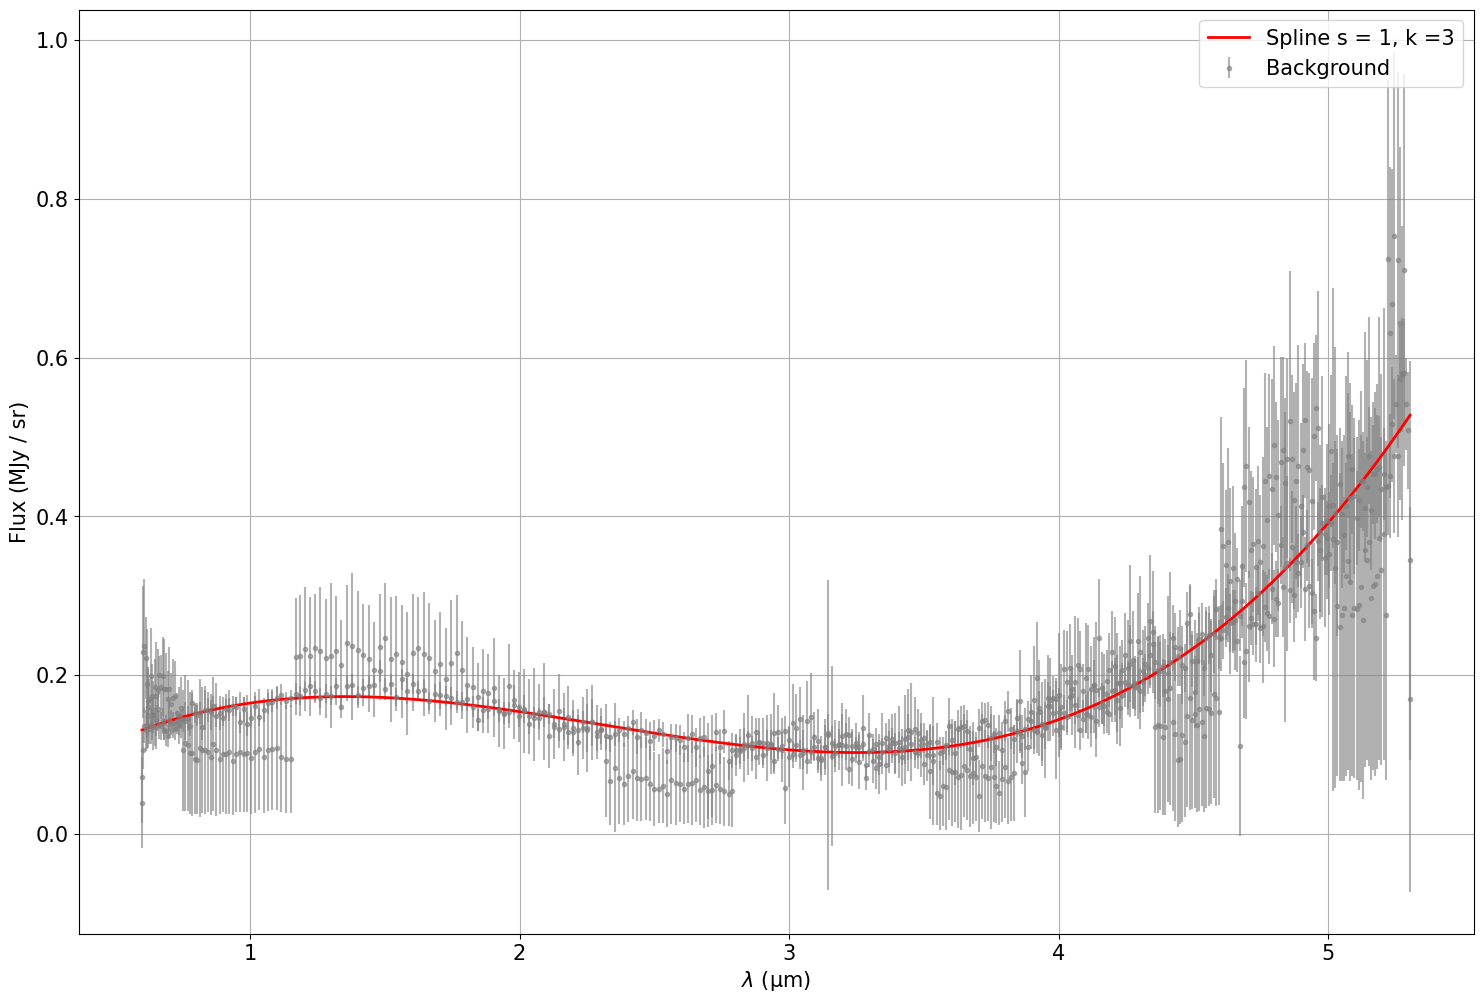
\includegraphics[scale=0.27]{assets/fit_spline.png}
  \caption{Extraction des spectres de fond sélectionnés sur la figure \ref{fig:extraction}, la spline ajustée est affichée en rouge. On remarque cependant que le nuage de points est séparé en 2 régimes, en raison du niveau de flux qui n'est pas le même sur une bande que sur l'autre.}
  \label{fig:spline_fit}
\end{wrapfigure}

À présent que l'on dispose d'un ensemble de points $(\lambda, z)$, on cherche à trouver une fonction approximant $z = f(\lambda)$ de façon à ignorer les variations rapides et le bruit. Pour cela, on utilise la fonction \textit{UnivariateSpline} du module \textit{SciPy.interpolate}, afin d'ajuster un modèle de spline à nos données. Puisque les variations qui nous intéressent sont les basses fréquences, et que celles ci peuvent parfois présenter plusieurs extrema, on choisira comme ordre de la spline le degré maximal, à savoir $k=5$ (cela signifie que les morceaux de polynômes servant à construire la courbe seront au plus de degré 5). 

On dispose également d'un paramètre de lissage $s \geq 0$, qui quantifie le nombre de sous intervalles sur lesquels on définit les morceaux de polynômes. Plus $s$ est proche de 0, plus la fonction passera proche de chaque point, plus $s$ est grand, plus la fonction sera "lisse" et ne suivra que l'allure générale de la distribution des points. On choisit, assez arbitrairement, une valeur de $s=0.01$.

Il est possible que dans certains cas, l'ajustement de la spline échoue. L'algorithme baisse alors la valeur de $k$ à $k=3$ et augmente la valeur de $s$ par facteurs de 10 jusqu'à obtenir un ajustement. C'est notamment le cas sur la figure \ref{fig:spline_fit} ($s=1$, $k=3$), où en raison des écarts entre les flux des 2 bandes de fond, l'ajustement a échoué.


\subsubsection{Aparté : Autres modèles d'ajustements}

\begin{wrapfigure}{l}{0.4\linewidth}
  \centering
  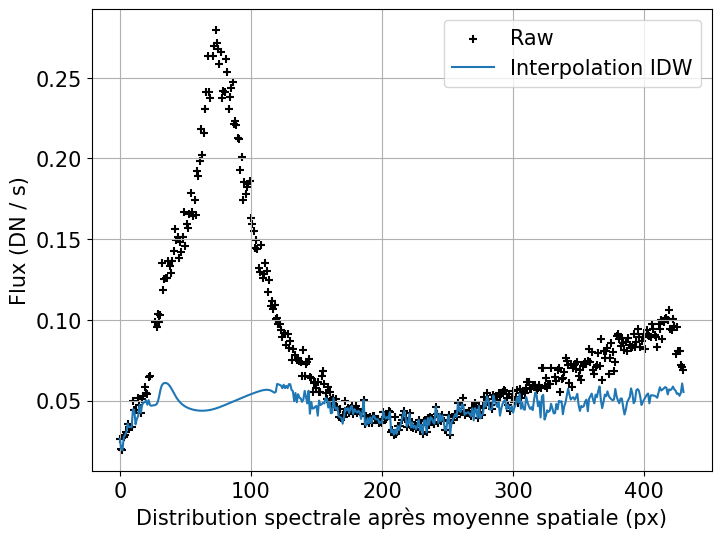
\includegraphics[scale=0.3]{assets/idw_interpolation.png}
  \caption{Moyenne spatiale du profil spectral d'une bande de fond, ainsi que d'une interpolation de ce même fond. On voit que les valeurs trop élevées sont tronquées, et que l'allure du profil n'est plus du tout suivie.}
  \label{fig:interpolation}
\end{wrapfigure}

Avant d'arriver au modèle actuel, plusieurs autres méthodes ont été envisagées et testées pour modeliser le fond.\\

Tout d'abord, les premiers tests ont été réalisés avant que l'étape de précalibration soit implémentée. Ceux ci avaient donc lieu sur des images non traitées par un champ plat.

Une première méthode naïve consiste en l'extraction des bandes 2D de fond, le rejet des pixels au-dessus d'un certain seuil (garder les 50\% des plus lumineux, rejeter ceux au-dessus de 70\% de la valeur maximale...), puis l'interpolation de ces pixels rejetés à partir des pixels restants. L'interpolation pondérée de distance avait alors été choisie, en raison de son paramètre de puissance qui offrait un certain contrôle sur le degré de lissage de l'interpolation. L'allure générale du fond est en revanche perdue (figure \ref{fig:interpolation}).\\

\begin{figure}[H]
  \centering
  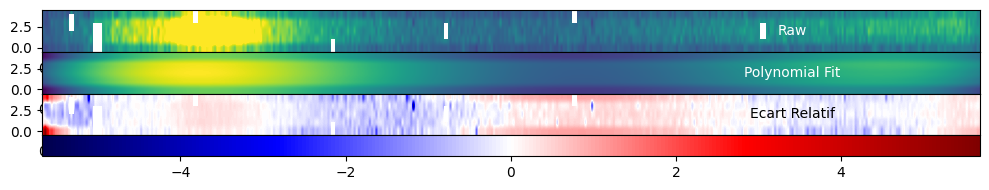
\includegraphics[scale=0.7]{assets/2D_polynomial.png}
  \caption{Comparaison entre données brutes d'une bande de fond (haut), un ajustement par un polynôme d'ordre 4 (milieu), et l'écart relatif $\frac{Raw - Fit}{Raw}$ (bas). Bien que l'allure générale semble suivie, des effets de bords importants sont visibles.}
  \label{fig:2D_polynomial}
\end{figure}

\begin{wrapfigure}{r}{0.6\linewidth}
  \centering
  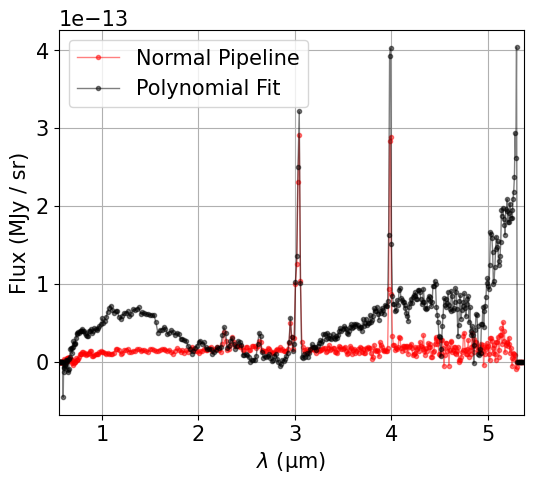
\includegraphics[scale=0.5]{assets/comparaison_normal_fit.png}
  \caption{Comparaison entre un spectre final obtenu par un traitement normal des données (rouge) et un spectre obtenu en ajustant le fond par des polynômes 2D}
  \label{fig:comparaison_fit_normal}
\end{wrapfigure}

Une autre stratégie consiste en l'ajustement d'un polynôme en 2 dimensions sur chaque bande de fond. Cependant, malgré des premiers résultats prometteurs (figure \ref{fig:2D_polynomial}), les rapides variations sur les bords de l'image induisent des écarts importants avec les spectres obtenus par le traitement par défaut du pipeline (figure \ref{fig:comparaison_fit_normal}).\\

Enfin, en raison du manque de temps, certains détails ont dû être ignorés. L'algorithme actuel peut encore être amélioré, notamment sur la sélection des bandes de fond et sur l'ajustement de la spline. En effet, la méthode actuelle ne permet pas de propager les incertitudes sur l'ajustement aux données après la soustraction. De plus, il existe encore certains cas limites pour lesquels l'ajustement échoue, ou alors des cas où la spline peut être trouvée, mais celle ci ne suit pas l'allure des données.


\subsubsection{Interpolation 2D et finitions}

Une fois notre spline $f(\lambda)$ obtenue, le spectre peut être interpolé en une image 2D à partir de la carte de longueurs d'ondes obtenue lors de la copie des données calibrées, à la fin de l'étape Photom. En effet, avant l'étape ResampleSpec, la direction de dispersion peut être légèrement déformée par rapport à l'axe horizontal. L'interpolation 2D a donc lieu avant cette étape afin de ne pas perdre d'informations lors du rééchantillonage inverse.

Les opérations mathématiques inverses de Photom, BarShadow, PathLoss et FlatField sont alors appliquées sur cette nouvelle image, donnant une image correspondant à une pseudo-observation du fond à travers les 3 fentes (figure \ref{fig:background}). Celle ci est alors soustraite à l'image originale, donnant une image finale sur laquelle on applique les étapes suivantes du pipeline.

\begin{figure}[H]
  \centering
  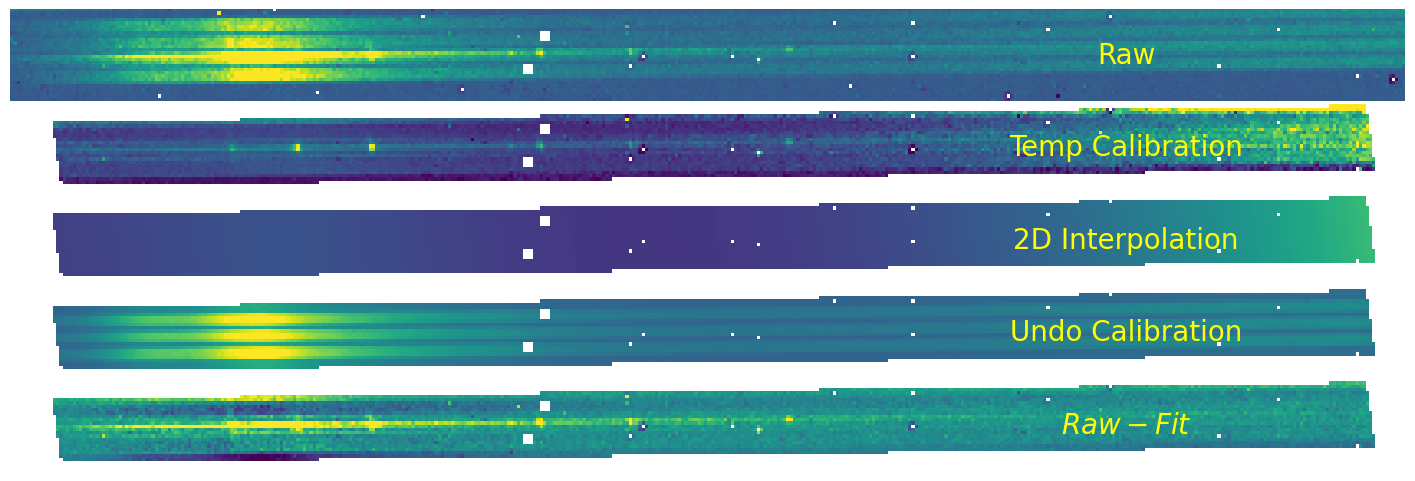
\includegraphics[scale=0.5]{assets/background_subtraction.png}
  \caption{Résumé des différentes opérations appliquées sur l'image d'une slitlet. De haut en bas on a : l'image pré-algorithme, l'image temporairement calibrée, une nouvelle image formée par un ajustement du fond et une interpolation 2D, cette même image décalibrée, la soustraction de l'image originale par l'image du fond}
  \label{fig:background}
\end{figure}

\subsection{Résultats}




\printnoidxglossaries

\printbibliography %Prints bibliography


\end{document}
